\documentclass[10pt]{article}
\usepackage[utf8]{inputenc}
\usepackage{kotex}
\usepackage{graphicx}
\usepackage{subfigure}
\usepackage{titling}
\setlength{\droptitle}{-2cm}
\usepackage{array}
\usepackage{amssymb}
\usepackage{amsmath}
\usepackage{siunitx} 
\usepackage{enumerate} 
\usepackage{pgfplots}
\usepackage{pgfplotstable}
\usepackage{tikz,pgfplots}
\usepackage{wasysym}
\usepackage{geometry}
\usepackage{authblk}
\usepackage{kotex}
\usepackage{bibunits}
\usepackage{tabularx}
\usepackage{hyperref}

\geometry{
    a4paper,
    total={170mm,257mm},
    left=20mm,
    top=20mm,
}

\title{\textbf{Artificial Intelligence: HW 2}}
\author{Jeong Min Lee}

\begin{document}
\maketitle

\section{HOG Feature Extraction}

In this section, I will introduce the results of \textbf{extract\_hog()}. The \textbf{extract\_hog()} function runs for at least 10 seconds for each image.

\begin{figure}[!h]
    \centering
    \subfigure[]{
        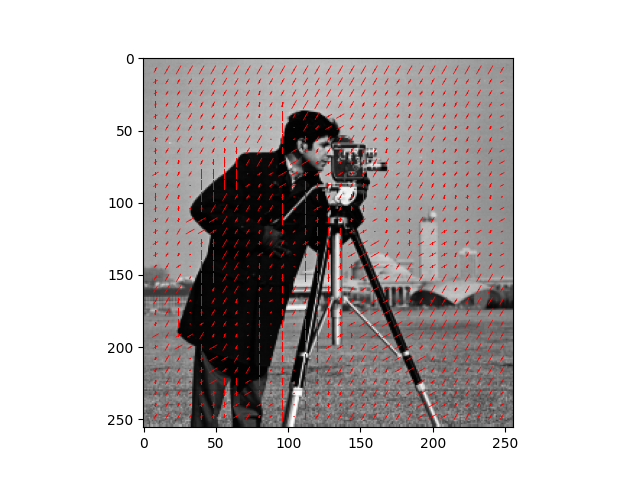
\includegraphics[scale=0.4]{../figures/hog1.png}
    }
    \subfigure[]{
        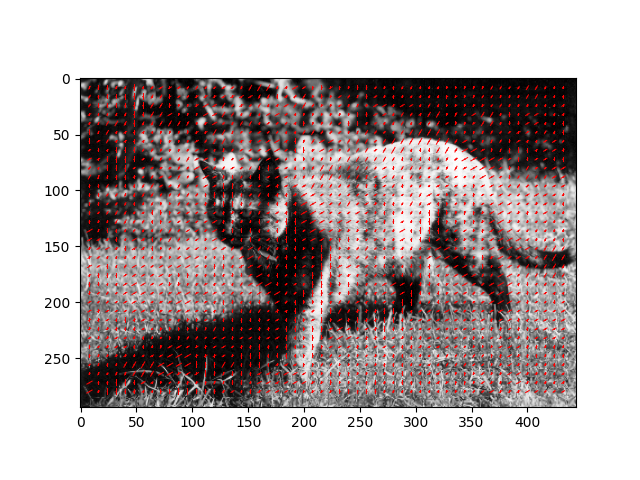
\includegraphics[scale=0.4]{../figures/hog2.png}
    }
    \subfigure[]{
        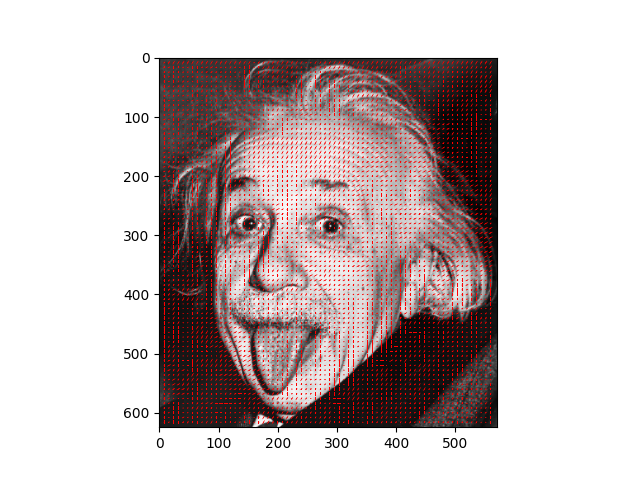
\includegraphics[scale=0.4]{../figures/hog3.png}
    }
    \subfigure[]{
        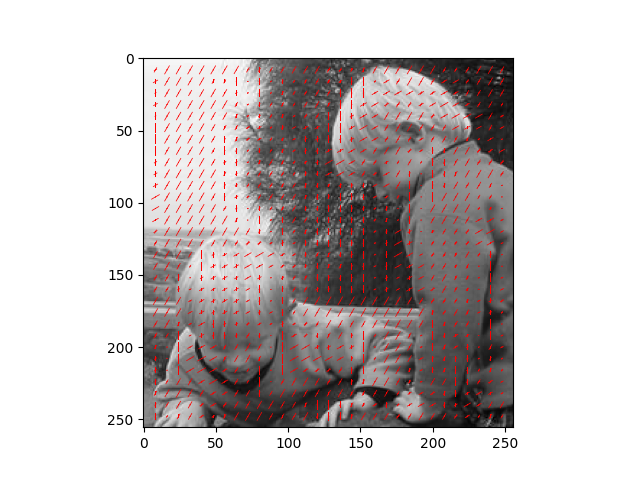
\includegraphics[scale=0.4]{../figures/hog4.png}
    }
    \caption{Results of HOG features extracted by \textbf{extract\_hog()}. Each HOG feature is derived from (a) cameraman.tif, (b) cat.tif, (c) einstein.png, (d) twins.tif.}
\end{figure}

\section{Face Detection}

In this section, I will present the results of \textbf{face\_recognition()}. I have implemented additional functions that were not specified in the original requirements: \textbf{non\_maximum\_suppression()} and \textbf{getIOU()}. These functions were introduced to enhance the readability and functionality of the code. Despite the efforts to optimize the code and reduce execution time, the process of creating the bounding box set remains a challenging task. The approximate running time of \textbf{face\_recognition()} and its visualization is approximately 13 minutes. We selected a threshold of 0.65 for the normalized cross-correlation (NCC) score based on empirical observations.

\begin{figure}[!h]
    \centering
    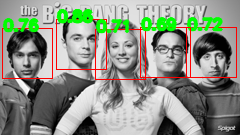
\includegraphics[scale=0.7]{../figures/result_face_detection.png}
\end{figure}

\end{document}
